% ICSOC 2026 submission -- Springer LNCS format
% Venue: https://icsoc2026.it.p.lodz.pl  (24th Int. Conf. on Service-Oriented Computing)
% Research papers: 10-15 pages incl. references, Springer LNCS, double-blind review.
% Build:  pdflatex paper && bibtex paper && pdflatex paper && pdflatex paper
% (requires llncs.cls and splncs04.bst, shipped alongside this file)
\documentclass[runningheads]{llncs}

\usepackage[T1]{fontenc}
\usepackage{graphicx}
\usepackage{amsmath}
\usepackage{amssymb}
\usepackage{mathtools}
\usepackage{booktabs}
\usepackage{xcolor}
\usepackage{algorithm}
\usepackage{algpseudocode}
\usepackage{tikz}
\usetikzlibrary{arrows.meta,positioning,calc,fit,backgrounds}
\usepackage{hyperref}
\renewcommand\UrlFont{\color{blue}\rmfamily}
\urlstyle{rm}
% allow long URLs to break across lines instead of overflowing the margin
\Urlmuskip=0mu plus 1mu\relax

\graphicspath{{figures/}}

\begin{document}

\title{Learning When to Stop:\\
A Deep Reinforcement Learning Service for Adaptive Shot Allocation in Quantum Circuit Execution}
\titlerunning{A DRL Service for Adaptive Shot Allocation in Quantum Circuits}

% Anonymised for double-blind review -- restore the author block for camera-ready.
\author{No Author Given}
\authorrunning{No Author Given}

\institute{No Institute Given}

\maketitle

\begin{abstract}
Quantum algorithms estimate output distributions by repeatedly sampling a circuit through \emph{shots}. Too few shots yield unreliable results, whereas too many waste costly quantum hardware time. We introduce a \emph{shot-allocation service}, an intermediary gateway that manages circuit execution and decides online, after each batch, when sufficient samples have been collected. Operating as a black box, the service requires no knowledge of circuit structure or backend noise. We formulate adaptive shot allocation as a Markov Decision Process and train a Deep Q-Network that observes nine features summarising the empirical distribution and chooses whether to continue or stop. The policy is trained using an asymmetric reward based on an a-posteriori optimal shot count derived from the point of diminishing returns, favouring slight overshooting over premature stopping. We evaluate the approach across hundreds of circuit-backend configurations, with separate training, model selection, and held-out evaluation sets. 
%The learned policy uses substantially fewer shots than worst-case a-priori bounds and achieves a lower mean deviation from the optimum than two of three state-of-the-art hand-tuned heuristics. 
Our results show that effective black-box shot allocation can be learned rather than manually designed.

\keywords{Quantum Computing \and Quantum Software Engineering \and
Service-Oriented Computing \and Shot Allocation \and Deep Reinforcement
Learning.}
\end{abstract}

\section{Introduction}
\label{sec:intro}

Quantum computation is inherently probabilistic: measuring a quantum circuit
collapses its state to a single classical outcome sampled from an unknown
probability distribution determined by the circuit and the hardware
noise~\cite{nielsen2010quantum}. To obtain a meaningful estimate of that
distribution, the same circuit must be executed many times; each repetition is a
\emph{shot}, and the empirical frequencies over many shots approximate the
underlying \emph{ground truth}.

\textit{How many shots are enough?} is a deceptively simple question that has a direct impact
on both the accuracy of the result and the cost of obtaining it. On today's
Noisy Intermediate-Scale Quantum (NISQ) devices~\cite{preskill2018nisq},
hardware time is scarce, expensive, and shared through queued cloud access, so
every redundant shot is wasted budget. Conversely, stopping too early produces
high-variance estimates and scientifically invalid conclusions. Practitioners
typically fix the shot count up front from rules of thumb, which is either
wasteful or unreliable because the right number depends on the specific circuit
and backend.\\
A recent line of work reframed this as the \emph{point of diminishing
returns}~\cite{bisicchia2026shots}: the moment at which additional shots no
longer meaningfully change the cumulative empirical distribution of a fixed
(static, non-variational) circuit. The idea is proposed as an online,
black-box procedure that executes shots in batches and stops once a
divergence-based stability criterion is met. While effective, such a procedure
embeds a hand-designed stopping rule whose sensitivity must be manually tuned.

In this paper we take a \emph{service-oriented} view of this problem. We propose a
\emph{shot-allocation service}: a lightweight intermediary, or gateway, that a
practitioner places between their application and the quantum cloud. The user
submits a circuit and a target accuracy; the service transparently drives its
execution on the chosen backend, monitors the stream of measurement outcomes
batch by batch, and decides online when the empirical distribution has stabilised
enough to stop, returning the result together with the number of shots actually
spent. The service treats the backend as a black box: it never inspects the
circuit structure or the noise model, only the statistics of the outcomes
observed so far.\\
%In this way it relieves practitioners of the brittle, circuit-specific tuning that fixing a shot count up front requires, and exposes shot optimisation as a reusable capability of the execution stack.
%The question we study is how the service should make its stop-or-continue decision. 
Rather than embedding a fixed convergence test, we let the service
\emph{learn} one: its decision logic is a \emph{Deep Reinforcement Learning}
(DRL) agent \cite{watkins1992qlearning}, trained on simulated executions, that discovers a stopping policy
from feedback on the quality of its decisions. This cleanly separates the
(expensive, offline) learning of the policy from the (cheap, online) decision that the deployed service performs.
% \paragraph{Design rationale.} Three choices shape the rest of the paper, and we
% state them up front so that later sections can refer back to them. First, the
% service is \emph{black-box}: it never inspects the circuit structure or the
% backend noise model, only the statistics of the outcomes it observes. This is
% what turns shot allocation into a reusable capability of the execution stack
% rather than a per-algorithm tool, and what lets the same service apply unchanged
% to any static circuit on any backend, at the cost of giving up the white-box
% signals that algorithm-specific methods exploit. Second, the stopping logic is
% \emph{learned} rather than hand-coded: instead of fixing a convergence test and
% tuning its thresholds over a grid, we let the agent discover the rule from
% feedback, so the machinery can be re-targeted (for instance to a different
% divergence) by retraining rather than redesign. Third, we package the result as
% a \emph{service}: the expensive learning happens once, offline, while the
% deployed gateway performs only the cheap per-batch stop-or-continue decision,
% transparently to the user.

\paragraph{Contributions.} The contributions of this work are:
\begin{enumerate}
  \item We cast black-box shot allocation as a \emph{service} that mediates
  between users and quantum-cloud backends. We package and release this service that wraps the learned policy behind a single execution
  endpoint (Section ~\ref{sec:deploy}).
  \item  To learn the service DRL model, we design a nine-feature state representation combining static problem
  descriptors with dynamic convergence signals built on the same
  diminishing-returns proxy that defines the Oracle, together
  with a precision-shaped asymmetric reward that encodes the domain-specific
  asymmetry between under- and over-sampling (Section~\ref{sec:method}).
  \item We train and evaluate the DRL service model on QSimBench~\cite{qsimbench} on
  hundreds of circuit backends  (testing is performed on held-out circuits, Sections~\ref{sec:setup}--\ref{sec:results}).
  %keeping a clean separation
  % between the instances used for training, those used to select the model
  % (validation), and a set of circuits held out for final evaluation only, and
  % we compare the learned policy against five reference methods on identical,
  % never-seen test circuits .
  % \item We provide a critical analysis of the learned behaviour, showing it is
  % robust and safety-oriented, uses orders of magnitude fewer shots than the
  % a-priori bounds, and achieves a lower mean deviation from the optimum than
  % two of the three divergence-based online policies
  % (Section~\ref{sec:results}).
\end{enumerate}

\section{Background and Related Work}
\label{sec:background}

\subsection{Quantum Circuits, Shots, and Noise}
\label{sec:qbackground}

A quantum circuit transforms a register of \emph{qubits} through a sequence of
gates and then measures them, returning a classical bit string in $\{0,1\}^m$
for $m$ qubits~\cite{nielsen2010quantum}. Measurement is intrinsically
probabilistic: a single execution does not reveal the underlying state but draws
one outcome from a probability distribution fixed by the circuit and the
hardware. For the purposes of this paper a measured circuit can therefore be
viewed as a randomised black box that, each time it is run, emits one classical
outcome.

Because one execution yields only one sample, a circuit must be run many times
to estimate its output distribution. Each repetition is a \emph{shot}, and the
empirical frequencies over $n$ shots, $\hat{P}_n(x)=\mathrm{count}_n(x)/n$,
approximate the underlying distribution, converging to it as $n$ grows. Shots
are not free, however: on cloud-accessed NISQ hardware~\cite{preskill2018nisq} they consume queued, billed device time,
and hardware noise (decoherence, gate and readout errors) perturbs the ideal
distribution, so past a certain point extra shots no longer reduce the dominant
error and only waste budget.
%The practical question is thus \emph{how many shots are enough}: stopping too early leaves the estimate dominated by sampling noise (\emph{undershooting}), while stopping too late wastes resources (\emph{overshooting}). Of the two, a small overshoot is the safer mistake, because an undershot estimate can be statistically invalid; we make this trade-off precise in the next subsection. 

We restrict attention to \emph{static}, non-variational circuits, whose gates
and parameters are fixed across all shots, so the effective output distribution
is stationary throughout an execution. This is distinct from variational
workloads, where a classical optimiser changes the circuit between iterations
and the distribution drifts; that setting requires different stopping criteria
and is outside our scope.

\subsection{The Shot-Allocation Problem and the Point of Diminishing Returns}

Let $P$ be the unknown distribution over the finite set of measurement outcomes
of a static circuit $C$ run on a backend $Q$, and let $\hat{P}_n$ be the
empirical distribution after $n$ shots. By the law of large numbers
$\hat{P}_n \to P$ almost surely, so for a divergence $\mathcal{D}(\cdot,\cdot)$
the deviation $\mathcal{D}(\hat{P}_n, P)$ vanishes as $n$ grows.

Since $P$ is inaccessible on real hardware, a recent
study~\cite{bisicchia2026shots} adopts an \emph{a-posteriori} reference: the
empirical distribution $\hat{P}_{\mathcal{B}}$ obtained under a fixed budget
$\mathcal{B}$. The a-posteriori optimal shot count is the smallest prefix length
$n^{\star}$ whose distribution is within a tolerance $\delta$ of the full-budget
reference, robustly to later fluctuations:
\begin{equation}
  n^{\star} = \min\bigl\{\, n \le \mathcal{B} \;\big|\;
  \mathcal{D}(\hat{P}_m, \hat{P}_{\mathcal{B}}) \le \delta \;\;\forall m \ge n \,\bigr\}.
  \label{eq:oracle}
\end{equation}
We use this quantity, computed by the suffix-stable Algorithm~1
of~\cite{bisicchia2026shots} with the Total Variation Distance (TVD), as our
\emph{Oracle}: the ground-truth label against which a stopping decision is
scored. Throughout, we fix $\mathcal{B}=20{,}000$ shots, a batch size of $50$,
and $\delta=0.10$.

\paragraph{Undershooting, overshooting, and the optimum.} The optimal stop
$n^{\star}$ is the fewest shots that already yield a result indistinguishable, up
to the tolerance $\delta$, from the full-budget estimate. Stopping at exactly
$n^{\star}$ is ideal but, under stochastic sampling, impossible to pinpoint, and
two failure modes flank it. \emph{Undershooting} means stopping at $n<n^{\star}$,
returning a distribution still dominated by sampling noise: the estimate is
statistically unreliable and any conclusion drawn from it may be invalid.
Instead, \emph{Overshooting} means stopping at $n>n^{\star}$, returning a result of essentially
the same quality as $n^{\star}$ but paying for the surplus $n-n^{\star}$ shots in
wasted device time. The two errors are therefore deeply \emph{asymmetric}: an
overshoot merely costs money, whereas an undershoot can invalidate the result.
A good stopping rule should accordingly err on the side of a slight overshoot,
and we build this preference directly into the reward (Section~\ref{sec:method}).

\subsection{Background: Reinforcement Learning and Deep Q-Networks}
\label{sec:background-dl}

Reinforcement learning (RL) models an agent that interacts with an environment
over discrete steps, choosing actions to maximise a cumulative
reward~\cite{sutton2018reinforcement}. The interaction is formalised as a
\emph{Markov Decision Process} (MDP) $(\mathcal{S},\mathcal{A},P,r,\gamma)$:
at step $t$ the agent observes a state $s_t\in\mathcal{S}$, takes an action
$a_t\in\mathcal{A}$, receives a reward $r_t$, and transitions to $s_{t+1}$
according to $P$. The goal is a policy $\pi$ maximising the expected discounted
return $\mathbb{E}\bigl[\sum_{k\ge 0}\gamma^{k} r_{t+k}\bigr]$, where
$\gamma\in[0,1)$ trades off immediate against future reward.

Q-learning~\cite{watkins1992qlearning} estimates the optimal action-value
function $Q^{\star}(s,a)$, the expected return of taking action $a$ in state $s$
and acting optimally thereafter, via the Bellman target
$y_t = r_t + \gamma\max_{a'}Q(s_{t+1},a')$. When the state space is large or
continuous, the lookup table is replaced by a neural function approximator
$Q(s,a;\theta)$, yielding the Deep Q-Network (DQN)~\cite{mnih2015human}, trained
by minimising the temporal-difference error $\bigl(y_t-Q(s_t,a_t;\theta)\bigr)$.
Two devices stabilise the otherwise unstable bootstrap of a function
approximator on its own predictions: \emph{experience replay}, which trains on
random mini-batches drawn from a buffer of past transitions to break temporal
correlations, and a periodically synchronised \emph{target network}, a frozen
copy of $\theta$ used to compute $y_t$.

\subsection{Related Work: Shot-Optimisation Strategies}
\label{sec:relwork}

Existing shot-optimisation methods for quantum circuits fall into four families,
which we review here and contrast with the present work.

\paragraph{A-priori concentration bounds.} Hoeffding-style~\cite{hoeffding1963}
and Weissman-style~\cite{weissman2003inequalities} inequalities provide
worst-case shot counts that guarantee a target deviation with high probability.
%They depend only on $\delta$, the confidence level, and the alphabet size, and
%are therefore independent of the actual circuit.
They usually are
extremely conservative, often overestimating the required shots by several
orders of magnitude.

\paragraph{Adaptive allocation for variational algorithms.} \emph{Variational} quantum
algorithms~\cite{cerezo2021vqa,kandala2017vqe} repeatedly updates circuit parameters via classic optimizers. iCANS allocates shots individually to each partial
derivative, spending more where the gradient signal is large relative to its
shot noise~\cite{kubler2020icans}; gCANS couples this choice across all
parameters to maximise the expected gain per shot, achieving geometric
convergence in convex regimes~\cite{gu2021gcans}; and Rosalin combines
per-derivative allocation with weighted random sampling of the Hamiltonian terms
to lower the cost of each energy estimate~\cite{arrasmith2020rosalin}. 
% related
% line keys the shot count to the entropy of the output distribution across
% iterations. All of these methods exploit algorithm-internal signals (gradients,
% Hamiltonian structure, an energy objective) and assume a non-stationary,
% iteration-driven workload; 
All these methods do not transfer to the static-circuit
setting we target, where the distribution is fixed and only the raw outcomes are
observable. 
%The two views are nonetheless complementary rather than mutually
%exclusive: within a single iteration the circuit parameters are held fixed and
%its output distribution is momentarily stationary, so our service can be applied
%\emph{independently at each iteration} to minimise the shots spent estimating
%that iteration's distribution, whatever scheme the outer optimiser uses to
%spread effort across iterations.

\paragraph{Learning-based methods.} 
% The strategy most related to ours uses
% machine learning, chiefly reinforcement learning (RL), to derive shot
% policies from execution data. Within variational workloads, an 
RL agents have been used to predicts shots across the iterations of classical optimisers~\cite{liang2024shotreduction}, and analogous RL controllers have been
proposed for recursive QAOA~\cite{rqaoa2026rlshots}. Supervised, epoch-based
schedules have likewise accelerated training in quantum machine
learning~\cite{phalak2023shot}. These approaches share the use of a learned
controller but differ from the present work in two aspects. \emph{(i) Workload:} they target \emph{non-stationary}, variational or
adaptive pipelines in which the circuit changes across iterations.
%, whereas we
%address \emph{static}, non-variational circuits with a fixed output
%distribution.
\emph{(ii) Observability:} they do not satisfy the black-box constraint, as they required explicit information (e.g., energies or gradient variances).
% \emph{(iii) Supervision and output:} their reward is the downstream
% task objective, so the learned policy is an \emph{allocator} tightly bound to
% one algorithm family; our only supervision is an a-posteriori optimal stop
% derived from the point of diminishing returns, so the learned policy is a
% \emph{general stopping rule} transferable across circuit families.
To our
knowledge, RL has not previously been used to learn a black-box stopping rule
for static-circuit shot allocation.

\paragraph{Online black-box control.} Online,
black-box frameworks~\cite{bisicchia2026shots,chen2024shotqc}  detect the point of
diminishing returns from the observed outcomes alone. Its behaviour is governed
by pluggable stopping, stability, and allocation policies; its best
configurations (denoted \mbox{Inc-TVD}, \mbox{Inc-Hell}, \mbox{Inc-JS}
according to the divergence used) constitute the state-of-the-art for static
circuits. Our work keeps the same black-box assumption but replaces the
hand-crafted, grid-tuned stopping rule with a \emph{learned} one, turning a
fixed convergence test into a trainable decision policy.

\section{Method}
\label{sec:method}

\subsection{System Architecture}

We first describe the system from the outside, as a service (Fig.~\ref{fig:service}),
and then open it up to show how its decision policy is learned.

\paragraph{The service.} The shot-allocation service is an intermediary that sits
between a user and a quantum-cloud backend. The user interacts with it through a
single request: they submit the circuit $C$ to run, the identifier of the
backend $Q$ to run it on, and a target accuracy $\delta$, and they receive back
the estimated output distribution and the number of shots actually spent. The
user supplies \emph{only} this input; they do not configure any stopping rule,
threshold, or shot count, and they are not involved in training the policy. From
the user's side the service is therefore a drop-in replacement for ``run this
circuit for a fixed number of shots'', except that the shot count is decided for
them. Internally, the service forwards $C$ to the chosen backend, executes it one
batch of shots at a time, and after each batch inspects the updated empirical
distribution to decide whether to request another batch or to stop. The service
never inspects the circuit or the noise model: from its viewpoint the backend is
a black box that, given a batch, returns measurement outcomes. Its single
non-trivial decision, \emph{continue or stop}, is precisely the stopping policy
this paper learns.

\begin{figure}[t]
\centering
\resizebox{\textwidth}{!}{%
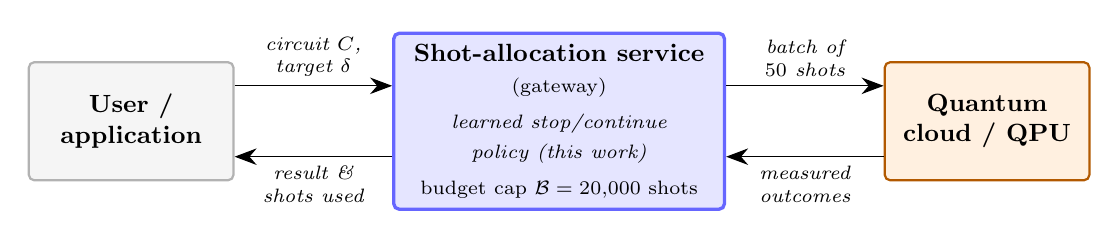
\begin{tikzpicture}[
  font=\small,
  box/.style={rounded corners=2pt, draw, thick, align=center,
              minimum height=15mm, inner sep=4pt},
  user/.style={box, fill=gray!8, draw=gray!60, minimum width=26mm},
  svc/.style ={box, fill=blue!10, draw=blue!60, very thick, minimum width=42mm},
  qpu/.style ={box, fill=orange!12, draw=orange!70!black, minimum width=26mm},
  lbl/.style={font=\scriptsize\itshape, align=center},
  >={Stealth[length=2.8mm]}
]
  \node[user] (user) {\textbf{User /}\\\textbf{application}};
  \node[svc, right=20mm of user] (svc) {\textbf{Shot-allocation service}\\{\scriptsize (gateway)}\\[2pt]{\scriptsize\itshape learned stop/continue}\\{\scriptsize\itshape policy (this work)}\\[2pt]{\scriptsize budget cap $\mathcal{B}=20{,}000$ shots}};
  \node[qpu, right=20mm of svc] (qpu) {\textbf{Quantum}\\\textbf{cloud / QPU}};

  \draw[->] ([yshift=4.5mm]user.east) -- node[lbl, above]{circuit $C$,\\target $\delta$} ([yshift=4.5mm]svc.west);
  \draw[->] ([yshift=-4.5mm]svc.west) -- node[lbl, below]{result \&\\shots used} ([yshift=-4.5mm]user.east);
  \draw[->] ([yshift=4.5mm]svc.east) -- node[lbl, above]{batch of\\$50$ shots} ([yshift=4.5mm]qpu.west);
  \draw[->] ([yshift=-4.5mm]qpu.west) -- node[lbl, below]{measured\\outcomes} ([yshift=-4.5mm]svc.east);
\end{tikzpicture}}
\caption{The shot-allocation service as an intermediary gateway between the user
and the quantum cloud. The user submits a circuit and a target accuracy; the
service drives execution on the backend one batch at a time, watches the returned
outcomes, and decides online when to stop, returning the estimated distribution
and the number of shots spent. Execution proceeds in batches of $50$ shots up to
a hard cap of $\mathcal{B}=20{,}000$ shots, the total budget beyond which the
service always stops. This paper concerns the service's stop/continue policy,
which is \emph{learned}.}
\label{fig:service}
\end{figure}

\paragraph{Inside the service: learning the policy.} The stop/continue policy is
obtained by reinforcement learning. At training time the service is embedded in a
standard RL loop of three conceptually distinct components. The \emph{agent} is
the DQN learner that, at each step, observes a compact state and chooses to
\textsc{continue} or to \textsc{stop}; it is the component that is eventually
distilled into the deployed service. The \emph{quantum environment} is a
simulated playground, built on QSimBench, that stands in for the backend: it
executes batches of shots and exposes the running statistics of the outcomes. The
\emph{Oracle} is a direct implementation of the a-posteriori optimum of
Eq.~\eqref{eq:oracle}; it is a training-time teacher whose answer is used
\emph{only} at the end of an episode to score the agent, and is never revealed
during decision making nor needed once the service is deployed.

\subsection{Deploying the Service}
\label{sec:deploy}

\paragraph{A pre-trained model that an operator can update.} Learning the policy
is a one-off, offline cost (Section~\ref{sec:setup}); the artefact that ships is
the trained policy network. The service is therefore delivered \emph{ready to
use}: an end user never trains anything and only issues execution requests.
Keeping the policy current is instead the responsibility of an
\emph{administrator} (operator) role, which can retrain the agent on new circuit
families or backends and hot-swap the deployed network, for instance to track
changing hardware or to adopt a different optimality criterion. This separation,
a user who only submits circuits and an administrator who owns the model, mirrors
how any trained-model-as-a-service component is operated.

\paragraph{Backend: CPU simulation today, a real QPU by configuration.} In this
work the backend $Q$ is not a physical quantum processor: we use QSimBench~\cite{qsimbench}, which
replays pre-computed shot-level traces on the CPU, to emulate execution cheaply
and reproducibly (Section~\ref{sec:dataset}). The service is agnostic to this
choice. Because it treats the backend purely as a source of measurement outcomes,
moving from emulation to real hardware is a matter of changing a single backend
parameter, from a QSimBench identifier to a quantum-cloud endpoint, with no change
to the learned policy or the surrounding logic.

%\paragraph{Exposing the service as a REST API.} Concretely, the gateway is a thin REST service: we wrap it in a minimal Flask application that accepts a circuit and a target backend on a single \texttt{POST /execute} endpoint and returns the estimated distribution and the shots spent as JSON (Fig.~\ref{fig:api}). The whole service is packaged as a Docker image, so a practitioner can stand it up next to their application as a single container. Because a real execution can take a long time, dominated by quantum-cloud queueing and the batches themselves rather than by the policy, a production deployment would expose this as an asynchronous job (submit, then poll for the result) rather than a single blocking call; we keep the synchronous form here for clarity.

%\begin{figure}[t]
%\centering
%\begin{minipage}{0.92\textwidth}
%\footnotesize
%\begin{verbatim}
%# Flask gateway: submit a circuit, get back result + shots used
%@app.route("/execute", methods=["POST"])
%def execute():
%    req = request.get_json()          # {algorithm, size, backend, delta}
%    dist, shots = service.run(
%        circuit=req["algorithm"], size=req["size"],
%        backend=req["backend"],       # QSimBench id today; a QPU by config
%        delta=req.get("delta", 0.10)) # target accuracy
%    return jsonify({"distribution": dist, "shots_used": shots})
%\end{verbatim}
%\end{minipage}
%\caption{Minimal REST interface to the service. A single \texttt{POST /execute} call takes a circuit specification and a target backend and returns the estimated output distribution together with the number of shots the learned policy decided to spend. Under QSimBench the circuit is given as a benchmark identifier (algorithm and size); on real hardware the same endpoint accepts the circuit itself. The container runs unchanged against an emulated or a real backend.}
%\label{fig:api}
%\end{figure}

\subsection{Practical Applicability on Real Quantum Clouds}
\label{sec:applicability}

A natural concern is whether a gateway that issues many small, adaptive batches
is viable on real quantum clouds, where per-job queueing could erode the savings
it produces. Recent infrastructure makes it so. Session-based execution models,
such as IBM Quantum sessions, grant a continuous execution window in which
successive batches are dispatched with minimal latency and preserved hardware
state, exactly the access pattern our service needs. Reservation-based models
offered by other providers (e.g.\ IonQ, Rigetti, AWS Braket) similarly let a
client pre-book a dedicated window and issue many submissions without re-entering
the global queue. Both, together with job batching, cut the per-batch overhead to
the point where tight, feedback-driven execution loops are practical. The service
is moreover a natural fit for the hybrid quantum-classical runtimes built for
variational workloads: the scheduling and session machinery those runtimes
already provide is what an adaptive gateway consumes, and, as noted in
Section~\ref{sec:relwork}, the service can be invoked per-iteration inside such a
loop. In short, the deployment we describe is aligned with where quantum-cloud
execution is already heading, and where shaving unnecessary shots translates
directly into less queue time and lower cost.

\subsection{State Space}
\label{sec:state}

After $t$ batches the agent has run $N_t = 50\,t$ shots of an instance
$(\mathtt{alg},n,\mathtt{bk})$ (algorithm, number of qubits, backend) and holds
the running empirical distribution $\hat{P}_t$ over the outcomes seen so far. It
sees this as a nine-number vector, every entry rescaled to $[0,1]$:
\begin{equation}
\mathbf{s}_t = \bigl(\;
  \underbrace{a,\;\; n/15,\;\; b,\;\; N_t/\mathcal{B}}_{\text{static descriptors}},\;\;
  \underbrace{\tilde{H}_t,\;\; C_t,\;\; \rho^{(1)}_t,\;\; \rho^{(L)}_t,\;\; \varrho_t}_{\text{dynamic convergence signals}}
\;\bigr)\;\in\;[0,1]^{9}.
\label{eq:state}
\end{equation}
The four \emph{static} entries say what the agent is running and how far along it
is: $a=\mathrm{idx}(\mathtt{alg})/(A-1)$ and $b=\mathrm{idx}(\mathtt{bk})/(K-1)$
are index encodings of the algorithm and backend over the $A$ algorithms and $K$
backends seen in training, $n/15$ is the circuit size, and $N_t/\mathcal{B}$ is a
progress bar over the budget.

The five \emph{dynamic} signals, refreshed after every batch, tell it how close
$\hat{P}_t$ is to settling. With $\hat{P}_t(x)=\mathrm{count}_t(x)/N_t$:
\begin{align}
\tilde{H}_t &= \frac{1}{n}\Bigl(-\!\!\sum_{x}\hat{P}_t(x)\log_2 \hat{P}_t(x)\Bigr),
  & &\text{(Shannon entropy, normalised by $n$ bits)} \label{eq:entropy}\\
C_t &= \sum_{x}\hat{P}_t(x)^2,
  & &\text{(concentration / collision probability)} \label{eq:conc}\\
\rho^{(\ell)}_t &= \mathrm{TVD}\!\bigl(\hat{P}_t,\hat{P}_{t-\ell}\bigr)
  = \tfrac{1}{2}\!\sum_{x}\bigl|\hat{P}_t(x)-\hat{P}_{t-\ell}(x)\bigr|,
  & &\ell\in\{1,L\},\;\; L=10, \label{eq:rate}\\
\varrho_t &= \min\!\bigl(N_t/(1500\,n),\,1\bigr).
  & &\text{(size-relative progress)} \label{eq:relprog}
\end{align}
Entropy~\eqref{eq:entropy} and concentration~\eqref{eq:conc} together say how
peaked or flat the distribution is; entropy is divided by $n$ so it does not
saturate on wide circuits. The two rate-of-change terms~\eqref{eq:rate} are the
core of the state: $\rho^{(1)}_t$ measures how much $\hat{P}_t$ moved over the
last batch and $\rho^{(L)}_t$ over the last $L=10$ batches. The latter is exactly
the diminishing-returns proxy behind the Oracle of Eq.~\eqref{eq:oracle}, so the
agent can watch the very quantity its reward is built on, while $\rho^{(1)}_t$
gives a shorter, noisier view. The last term~\eqref{eq:relprog} rescales the shot
count by a size-dependent budget ($1500\,n$), helping the agent tell early noise
from genuine late convergence on larger circuits.

\subsection{Actions, Episodes, and Reward}

The agent has two actions: \textsc{continue} runs one more batch of $50$ shots
and updates the state, \textsc{stop} ends the episode (an episode also ends on
its own once the budget $\mathcal{B}$ is spent). Only the final action is
rewarded: the environment compares the agent's total shots to the Oracle's
$n^{\star}$ and returns a single terminal reward, while the pressure toward
fewer shots comes from discounting. The reward is deliberately \emph{asymmetric},
because the two mistakes are not equally bad, undershooting gives an invalid
result whereas overshooting only wastes shots, and \emph{precision-shaped}, so
the best score sits on a small overshoot plateau rather than on a knife-edge
perfect stop. With $\text{error} = n_{\text{agent}} - n^{\star}$ and a plateau
margin $m = 200$ shots,
\begin{equation}
  R_{\text{term}} =
  \begin{cases}
    \bigl(\beta - \tfrac{|\text{error}|}{n^{\star}}\bigr)\,\sigma,
      & \text{error} < 0 \quad (\text{undershoot}),\\[4pt]
    \exp\!\bigl(-\lambda\,\tfrac{\max(0,\,\text{error}-m)}{n^{\star}}\bigr),
      & \text{error} \ge 0 \quad (\text{overshoot}),
  \end{cases}
  \label{eq:reward}
\end{equation}
with decay rate $\lambda = 2$, $\sigma = 1 + 0.5\,n^{\star}/\mathcal{B}$ scaling
the penalty with difficulty, and $\beta = -1.85$ for \emph{small} instances
($n^{\star} \le 5{,}000$) or $-2.5$ for \emph{big} ones. Overshooting scores the
full reward anywhere in $[0,m]$ and then decays \emph{relative to} $n^{\star}$, so
the same absolute overshoot hurts a lot on a cheap circuit but little on an
expensive one; undershooting is treated as a flat failure with a large negative
reward. The net effect is a safety-first bias that still pulls the policy toward
the diagonal.

\subsection{Network and Learning Algorithm}

The $Q$-function is a multi-layer perceptron: nine inputs (the state of
Eq.~\eqref{eq:state}), three hidden ReLU layers of $512$, $256$, and $128$ units
($10\%$ dropout after the first two, switched off during action selection so the
greedy policy is deterministic), and two linear outputs for
$Q(s,\textsc{continue})$ and $Q(s,\textsc{stop})$. Training uses the standard DQN
target~\cite{mnih2015human},
$y_t = r_t + \gamma\,(1-d_t)\max_{a'}Q_{\bar\theta}(s_{t+1},a')$ with $d_t$ the
terminal flag, minimising the squared temporal-difference error
$\bigl(y_t - Q_\theta(s_t,a_t)\bigr)^2$. We use $\varepsilon$-greedy exploration
($\varepsilon$ decaying once per episode from $1.0$ to $0.05$), a replay buffer of
$200{,}000$ transitions, mini-batches of $64$, Adam at learning rate $10^{-4}$,
discount $\gamma = 0.997$, and a target network synced every $2{,}000$ gradient
steps.

\subsection{Dataset, Oracle Labels, and Data Split}
\label{sec:dataset}

We build on QSimBench~\cite{qsimbench}, an execution-level benchmark for quantum
software engineering. Rather than shipping only circuit definitions, it provides
more than 20 million \emph{precomputed shot-level traces}: for each (algorithm,
size, backend) it stores the actual outcome sequence of a full
$\mathcal{B}=20{,}000$-shot run. We can therefore replay realistic noisy
executions on the CPU, deterministically and at no hardware cost, which is what
makes a large, reproducible study of stopping policies possible. The suite spans
many algorithms (e.g.\ dj, qaoa, qft, vqe, qnn, random), sizes from $4$ to $14$
qubits, and five IBM noisy backend simulators (\texttt{fake\_fez},
\texttt{fake\_kyiv}, \texttt{fake\_marrakesh}, \texttt{fake\_sherbrooke},
\texttt{fake\_torino}). Each instance is a (algorithm, size, backend) triplet
whose Oracle label $n^{\star}$ is precomputed once via Eq.~\eqref{eq:oracle}.

We split the instances once, without overlap, into three roles: a \emph{training}
pool the agent learns from, a \emph{validation} pool used only for model selection
(Section~\ref{sec:setup}), and a \emph{test set} never seen during either. For a
leakage-free comparison with the state of the art, the test set is fixed to the
$36$ benchmark traces used by a recent study~\cite{bisicchia2026shots} (a balanced
mix of \emph{small}, $n<10$, and \emph{big}, $n\ge10$, circuits); the rest, after
dropping the \texttt{grover-noancilla} variants, form the training/validation
pool. Every number we report aggregates many independent executions: training
touches a different instance each episode, and each test instance is replayed many
times. Because outcomes are sampled stochastically, even a fixed argmax policy
takes a different trajectory each run, so we report mean$\pm$std behaviour
(Section~\ref{sec:setup}).

The available instances are heavily skewed toward \emph{small} circuits that
converge in few shots. To counter this, the \textsc{generic} agent studied here
trains on a balanced 50/50 mix of small ($n<10$) and big ($n\ge10$) problems, so
it sees the full range of convergence behaviours.

\section{Development and Experimental Setup}
\label{sec:setup}

We adopt the well-established DQN machinery (Section~\ref{sec:background-dl}) as
the learning backbone, with the network itself being a standard multi-layer
perceptron of ReLU units (Section~\ref{sec:method}).
The system is implemented in Python~3.12. The agent
and network use PyTorch~\cite{paszke2019pytorch}; the environment implements the
OpenAI Gym interface~\cite{brockman2016gym}; QSimBench supplies the circuit
traces and noise profiles. The full source code, oracle cache, and evaluation
scripts are released as open source; the repository is anonymised for
double-blind review at
\url{https://anonymous.4open.science/r/drl-shot-allocation}, with the
de-anonymised link to follow in the camera-ready version.\\
Each agent is trained from scratch with a fixed
random seed for reproducibility. The production \textsc{generic} agent is
trained for $1{,}000$ episodes, with the $\varepsilon$-greedy exploration rate
decaying once per episode (Section~\ref{sec:method}).\\
During model selection, we held out a
$20\%$ \emph{validation} set, disjoint from the 36
test traces and stratified by Oracle difficulty so that it mirrors the
distribution the agent trains on. We use the Mean Absolute Error (MAE) between the predicted shots and the target shots as selection metric, and we apply early stopping with $5$ patience steps.
%From episode $400$ onward the model is
%checkpointed every $100$ episodes and scored on this set by Mean Absolute Error
%(MAE) in shots; we keep the lowest-MAE checkpoint, apply early stopping with
%patience $5$, and restore the best-validation weights at the end. 
Because quantum
sampling makes a single validation pass noisy, each checkpoint's score is
averaged over \emph{three} stochastic passes of the whole validation set. 
% This protocol is motivated by the shape of
% the learning curve observed in an exploratory long-horizon run: training passes
% through an initial conservative ``stop-early'' phase, then a breakthrough in
% which the MAE drops sharply as circuit-specific stopping behaviour emerges, and
% finally an overfitting regime of hyper-conservative maximum-budget stops.
% De-noised, validation-MAE checkpointing retains the policy from the sweet spot
% between these extremes rather than the final (degraded) weights.
\paragraph{Evaluation protocol.} The selected agent is evaluated on the 36
held-out traces with a deterministic (greedy, $\arg\max_a Q$) policy. To capture
the stochasticity of quantum sampling we run a \emph{multi-run} evaluation: the
agent is replayed $N$ times per trace, and we report, per problem, the mean and
standard deviation of the shots used and of the resulting deviation from the
Oracle. The headline metric is the absolute deviation
$|n_{\text{agent}}-n^{\star}|$ in shots; we also report it as a percentage of the
budget $\mathcal{B}$.

\section{Results}
\label{sec:results}

\subsection{How the Agent Learns to Stop}

%Figure~\ref{fig:dashboard} summarises the training and evaluation of the
%\textsc{generic} agent. The reward moving average stabilises quickly while the
%MAE undergoes the sharp breakthrough decline described above, confirming that
%the learning is productive rather than a mere reward artefact. Because outcomes
%are stochastic and the test circuits are unseen, the agent cannot memorise a
%scalar shot count; to stop well it must interpret the dynamic state features,
%chiefly entropy, the concentration, and the two lag-based rates of change, to
%locate the point of stability.

% \begin{figure}[t]
% \centering
% \begin{minipage}[t]{0.49\textwidth}\centering
%   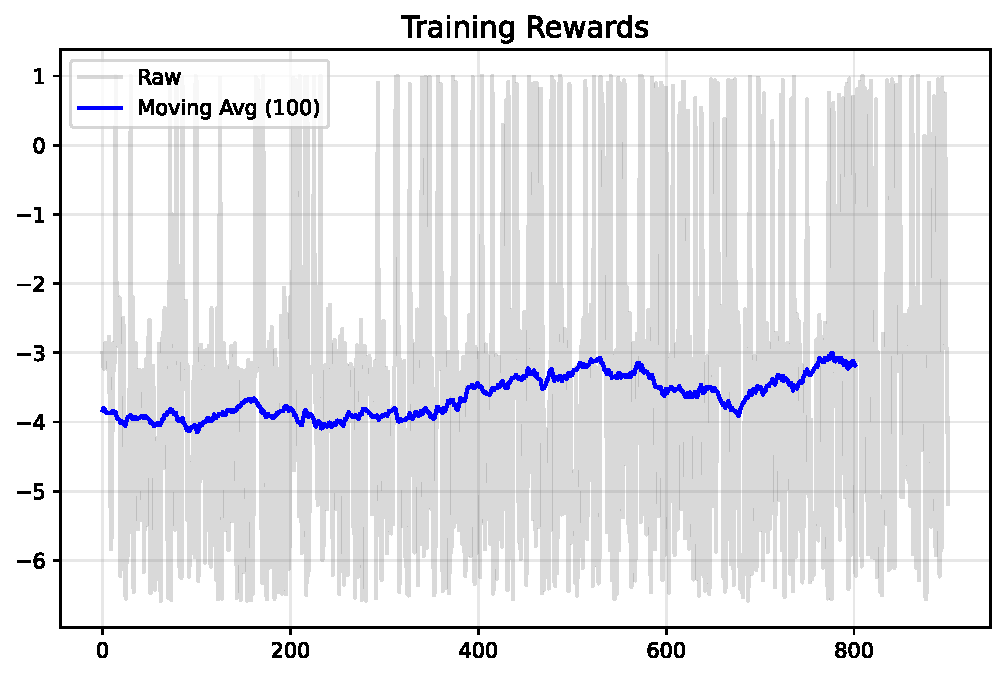
\includegraphics[width=\linewidth]{training_rewards.pdf}\\
%   {\footnotesize (a) Episodic training reward}
% \end{minipage}\hfill
% \begin{minipage}[t]{0.49\textwidth}\centering
%   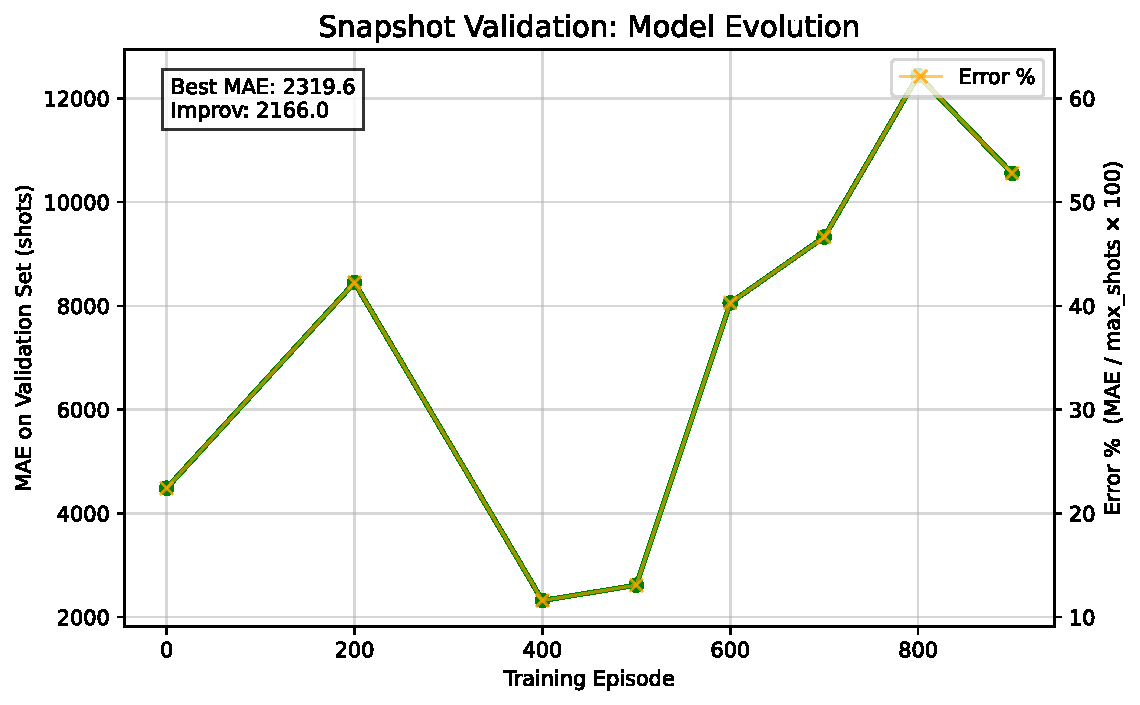
\includegraphics[width=\linewidth]{snapshot_validation.pdf}\\
%   {\footnotesize (b) Validation MAE across checkpoints}
% \end{minipage}
% \caption{Training and evaluation diagnostics for the \textsc{generic} agent.
% (a)~Episodic reward during training (raw trace and $100$-episode moving average),
% which stabilises early. (b)~Mean absolute error (MAE) on the validation set at
% each saved checkpoint, showing the sharp breakthrough decline that motivates the
% de-noised checkpoint selection of Section~\ref{sec:setup}.}
% \label{fig:dashboard}
% \end{figure}

Figure~\ref{fig:scatter} plots, for each held-out trace, the shots chosen by the
agent against the Oracle optimum. Points on the diagonal denote perfect stops,
points above denote (safe) overshooting, and points below denote (risky)
undershooting. The agent tracks the Oracle across the whole difficulty
spectrum, with a mean absolute deviation of $2{,}049$ shots ($10.2\%$ of the
budget), and it rarely undershoots ($3$ of $36$ traces, each by at most $200$
shots). Notably, the deviation is roughly balanced between the small and big
halves of the test set (mean MAE $2{,}108$ vs.\ $1{,}989$), and on the largest,
near-budget circuits (12--14-qubit \texttt{qft}/\texttt{random}, whose Oracle
already sits at $15$--$18$k shots) the agent stops within a few hundred shots of
the optimum. The residual error instead concentrates on \emph{mid-range}
instances (small-to-moderate Oracle values on $6$--$8$-qubit
\texttt{qaoa}/\texttt{qft}/\texttt{qnn} circuits), where the agent is
over-conservative and keeps sampling well past the diminishing-returns point,
spending two to four times the optimal shot count.

\begin{figure}[t]
\centering
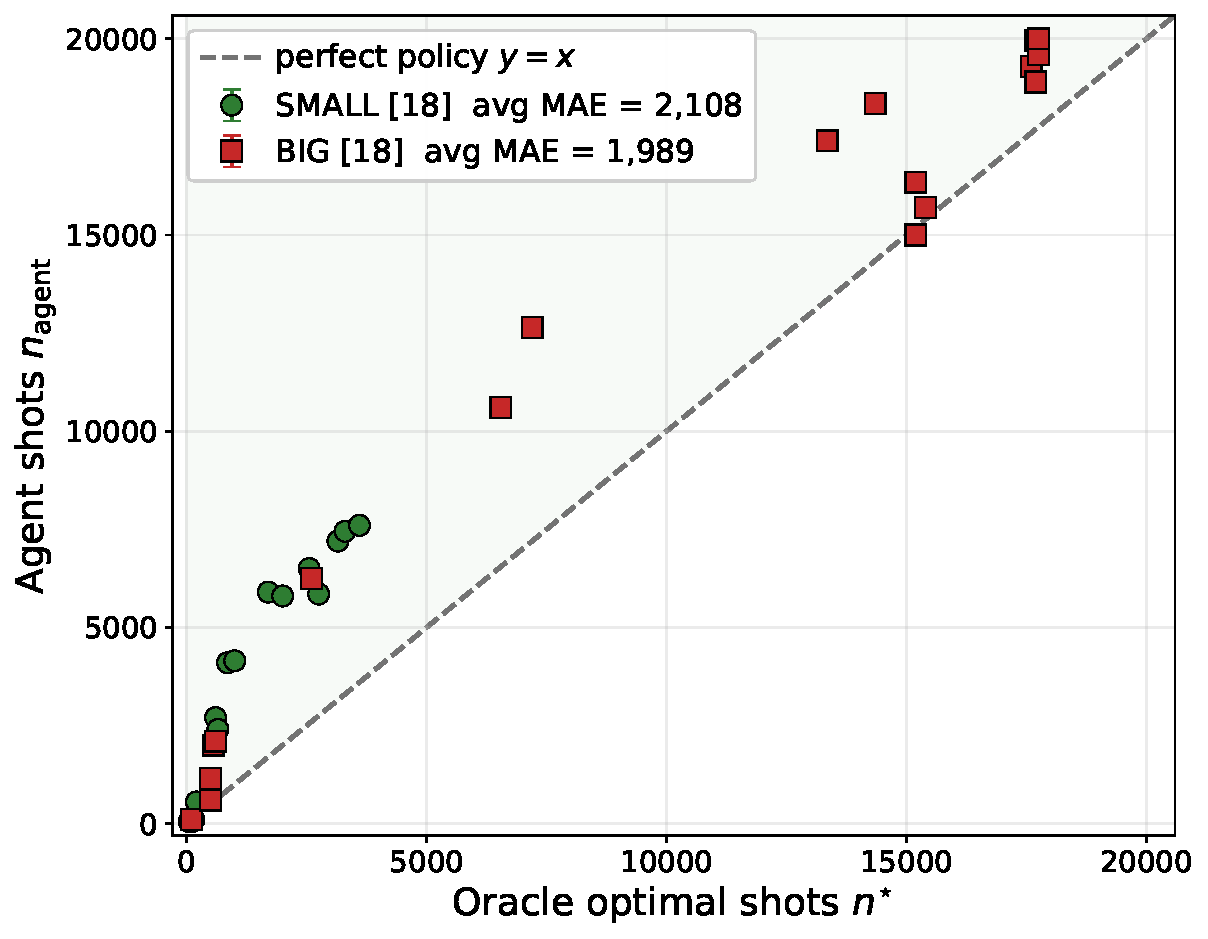
\includegraphics[width=0.8\textwidth]{agent_vs_oracle-generic-all36.pdf}
\caption{Agent policy vs.\ Oracle on the 36 held-out traces. The dashed line is
the perfect policy $y=x$.}
\label{fig:scatter}
\end{figure}

\subsection{Comparison with the State of the Art}

We compare the learned policy against five reference methods on the identical 36
traces at $\delta=0.10$: the three best online \textsc{IncrementalExecution}
configurations (\mbox{Inc-TVD}, \mbox{Inc-Hell}, \mbox{Inc-JS}) and the two
a-priori bounds (Weissman, Hoeffding)~\cite{bisicchia2026shots}. The full
per-trace breakdown is given in
Tables~\ref{tab:pertrace-small}--\ref{tab:pertrace-large}; we summarise the
aggregate comparison in prose below.

% AUTO-GENERATED by make_tables.py -- do not edit by hand.
% Re-run paper/make_tables.py to refresh after a new evaluation.

\begin{table}[t]
\centering
\footnotesize
\setlength{\tabcolsep}{4pt}
\caption{Per-trace shot counts on the \emph{small} circuits ($n<10$): a-posteriori Oracle, the proposed DRL agent (mean over evaluation runs), and the online Inc-* policies / a-priori Weissman bound of the reference framework~\cite{bisicchia2026shots} at $\delta=0.10$.}
\label{tab:pertrace-small}
\begin{tabular}{lccrrrrr}
\toprule
Trace & $n$ & Oracle & DRL (ours) & Inc-TVD & Inc-Hell & Inc-JS & Weissman \\
\midrule
dj\_4\_FEZ & 4 & 50 & 50 & 150 & 700 & 700 & 705 \\
dj\_4\_TOR & 4 & 50 & 50 & 150 & 550 & 500 & 705 \\
qaoa\_4\_SHE & 4 & 150 & 100 & 150 & 1300 & 900 & 705 \\
qaoa\_6\_MAR & 6 & 650 & 2{,}400 & 1450 & 1950 & 2400 & 2{,}368 \\
qft\_6\_TOR & 6 & 850 & 4{,}100 & 2050 & 1950 & 2600 & 2{,}368 \\
qft\_6\_FEZ & 6 & 1000 & 4{,}150 & 1750 & 1800 & 2500 & 2{,}368 \\
random\_6\_FEZ & 6 & 600 & 2{,}700 & 1700 & 1800 & 2600 & 2{,}368 \\
vqe\_6\_KYI & 6 & 50 & 50 & 150 & 1450 & 1500 & 2{,}368 \\
dj\_8\_MAR & 8 & 50 & 50 & 150 & 1400 & 2000 & 9{,}023 \\
dj\_8\_FEZ & 8 & 100 & 50 & 550 & 2300 & 1900 & 9{,}023 \\
qaoa\_8\_SHE & 8 & 1700 & 5{,}900 & 2300 & 4150 & 4600 & 9{,}023 \\
qaoa\_8\_KYI & 8 & 2000 & 5{,}800 & 2350 & 4150 & 5400 & 9{,}023 \\
qft\_8\_FEZ & 8 & 3300 & 7{,}450 & 3650 & 3300 & 4900 & 9{,}023 \\
qft\_8\_TOR & 8 & 3600 & 7{,}600 & 3500 & 3350 & 4800 & 9{,}023 \\
qnn\_8\_FEZ & 8 & 2550 & 6{,}500 & 3100 & 3700 & 5000 & 9{,}023 \\
qnn\_8\_KYI & 8 & 3150 & 7{,}200 & 3550 & 3500 & 4500 & 9{,}023 \\
random\_8\_FEZ & 8 & 2750 & 5{,}850 & 3100 & 3600 & 5300 & 9{,}023 \\
vqe\_8\_KYI & 8 & 200 & 550 & 1100 & 2700 & 2700 & 9{,}023 \\
\bottomrule
\end{tabular}
\end{table}

\begin{table}[t]
\centering
\footnotesize
\setlength{\tabcolsep}{4pt}
\caption{Per-trace shot counts on the \emph{big} circuits ($n\ge10$): a-posteriori Oracle, the proposed DRL agent (mean over evaluation runs), and the online Inc-* policies / a-priori Weissman bound of the reference framework~\cite{bisicchia2026shots} at $\delta=0.10$.}
\label{tab:pertrace-large}
\begin{tabular}{lccrrrrr}
\toprule
Trace & $n$ & Oracle & DRL (ours) & Inc-TVD & Inc-Hell & Inc-JS & Weissman \\
\midrule
dj\_10\_FEZ & 10 & 100 & 100 & 1600 & 3450 & 4200 & 35{,}600 \\
dj\_10\_TOR & 10 & 500 & 600 & 2200 & 4450 & 4700 & 35{,}600 \\
qaoa\_10\_SHE & 10 & 6550 & 10{,}600 & 9950 & 9750 & 11000 & 35{,}600 \\
qaoa\_12\_MAR & 12 & 7200 & 12{,}650 & 9000 & 14950 & 15900 & $1.42e{+}5$ \\
qft\_12\_TOR & 12 & 15200 & 16{,}350 & 17200 & 19350 & 20000 & $1.42e{+}5$ \\
qft\_12\_FEZ & 12 & 15400 & 15{,}700 & 17150 & 18150 & 20000 & $1.42e{+}5$ \\
random\_12\_FEZ & 12 & 15200 & 15{,}000 & 17100 & 19250 & 20000 & $1.42e{+}5$ \\
vqe\_12\_KYI & 12 & 550 & 2{,}000 & 3400 & 6150 & 7500 & $1.42e{+}5$ \\
dj\_14\_FEZ & 14 & 500 & 1{,}150 & 2450 & 4850 & 5200 & $5.68e{+}5$ \\
dj\_14\_MAR & 14 & 600 & 2{,}100 & 2300 & 5150 & 6200 & $5.68e{+}5$ \\
qaoa\_14\_KYI & 14 & 13350 & 17{,}400 & 13400 & 20000 & 20000 & $5.68e{+}5$ \\
qaoa\_14\_SHE & 14 & 14350 & 18{,}350 & 14600 & 20000 & 20000 & $5.68e{+}5$ \\
qft\_14\_FEZ & 14 & 17750 & 19{,}600 & 17800 & 20000 & 20000 & $5.68e{+}5$ \\
qft\_14\_TOR & 14 & 17750 & 20{,}000 & 17750 & 20000 & 20000 & $5.68e{+}5$ \\
qnn\_14\_FEZ & 14 & 17600 & 19{,}300 & 17700 & 20000 & 20000 & $5.68e{+}5$ \\
qnn\_14\_KYI & 14 & 17700 & 19{,}950 & 17750 & 20000 & 20000 & $5.68e{+}5$ \\
random\_14\_FEZ & 14 & 17700 & 18{,}900 & 17800 & 20000 & 20000 & $5.68e{+}5$ \\
vqe\_14\_KYI & 14 & 2600 & 6{,}250 & 4500 & 11150 & 14000 & $5.68e{+}5$ \\
\bottomrule
\end{tabular}
\end{table}


Two findings stand out. First, the learned agent is overwhelmingly more
efficient than the a-priori bounds: Weissman and Hoeffding overshoot the Oracle
by roughly two and seven \emph{orders of magnitude} respectively, because they
must hold for the worst case over all distributions, whereas the agent adapts to
the observed statistics. Second, among the divergence-based online policies, the agent's mean deviation
of $2{,}049$ shots is $1.3\times$ lower than that of \mbox{Inc-Hell}
($2{,}706$) and $1.6\times$ lower than that of \mbox{Inc-JS} ($3{,}336$), while
\mbox{Inc-TVD} records $871$, a configuration selected from an exhaustive grid
of hand-tuned configurations specifically for this metric. The agent achieves
this level of performance \emph{without} any hand-crafted stopping rule,
learning the stopping logic purely from data.

\subsection{Discussion}

\paragraph{Strengths.} (i)~\emph{Black-box generality}: the policy is driven only
by observed outcome statistics, with no access to the circuit or noise model, and
generalises to circuit families held out from training. (ii)~\emph{Safety-first
behaviour}: the asymmetric reward yields error distributions that are right-skewed
(the agent prefers a few extra shots to a premature, invalid stop), which is the
desirable bias in a scientific setting. (iii)~\emph{Modularity}: since the policy
is learned from the Oracle's signal rather than hard-coded, swapping the Oracle's
divergence (TVD $\to$ Hellinger/JS) only requires retraining, not redesign.

\paragraph{Implications for the service.} These properties are what let the
result be operated as a service rather than a one-off experiment. Because the
policy is black-box and reads only outcome statistics, a single deployed gateway
serves \emph{any} static circuit on \emph{any} backend with no per-circuit
tuning; because it ships as a pre-trained network behind a thin REST API
(Section~\ref{sec:deploy}), a call costs one request and the per-batch decision
is negligible next to the quantum execution it governs; and because the behaviour
is safety-first, the service can be trusted to err toward a few extra shots
rather than return an invalid result, which is the right default for an
unattended intermediary. The same modularity means an operator can re-tune the
service (a different divergence, a different cost trade-off) by retraining,
without touching the deployment.

\paragraph{Limitations.} The agent's dominant error mode is conservative
\emph{overshooting on mid-range circuits}: on $6$--$8$-qubit \texttt{qaoa}/\texttt{qft}/\texttt{qnn}
instances whose diminishing-returns point lies a few thousand shots in, the
agent keeps sampling and stops two to four times too late. By contrast, it
handles both extremes well: trivially short circuits and the largest,
near-budget circuits are stopped tightly. Undershooting, the scientifically
dangerous failure mode, is nearly eliminated ($3/36$, each within $200$ shots).
The over-conservatism is consistent with a value function that overestimates the
return of continuing; this points to two levers for further tightening the
learned stops: sharper reward shaping in the mid-range, and richer
mid-range convergence descriptors (e.g.\ an explicit convergence-streak feature
and overestimation-robust value learning) that we leave to future work.

\paragraph{Threats to validity.} \emph{Construct validity.} We score against an a-posteriori Oracle rather than the
inaccessible true distribution; this is the same principled reference used by the
state of the art~\cite{bisicchia2026shots}, and we use the identical $\delta$,
budget, and batch size for comparability. \emph{Internal validity.} Quantum
sampling is stochastic; we mitigate run-to-run variance through multi-run
evaluation and fixed seeds. \emph{External validity.} Experiments use IBM noisy
\emph{simulators} from QSimBench rather than live hardware, and target static,
non-variational circuits; transfer to real devices and to variational workloads
remains future work.

\section{Conclusion and Future Work}
\label{sec:conclusion}

We presented a \emph{shot-allocation service}, an intermediary gateway between a
user and the quantum cloud, whose decision logic is a Deep Reinforcement Learning
agent that learns, under a strict black-box assumption, when to stop sampling a
quantum circuit. Framed as a Markov Decision Process with a nine-feature state and
a precision-shaped, safety-oriented asymmetric reward, the agent learns a stopping
policy that generalises to unseen circuit families, uses far fewer shots than
a-priori concentration bounds, and achieves a lower mean deviation from the
optimum than two of the three hand-tuned online heuristics that represent the
state of the art, all without encoding any explicit convergence test.
The result is a lightweight, pre-trained policy network that ships behind a thin
REST API and runs unchanged against an emulated or a real backend. This
establishes that black-box shot allocation can be \emph{learned} rather than
hand-designed.

Future work targets further improvements to the learned policy: sharper
reward shaping for the mid-range circuits the agent currently over-samples,
enriching the state with additional convergence descriptors, overestimation-robust
value learning (e.g.\ Double DQN) and distributional RL variants, and ultimately
validating on live quantum hardware and extending the formulation toward
variational workloads.

\section*{Artifact Availability and Reproducibility Statement}

The anonymized replication package is available at
\textcolor{red}{METTERE QUI IL LINK ALLA REPO ANONIMIZZATA E COMPLETARE COSA C'E'}
\url{LINK}. It includes the scripts used to... (e.g. codice del servizio, del modello, dati di training, script per generare i plot, etc.)

\bibliographystyle{splncs04}
\bibliography{references}

\end{document}
